\documentclass[12pt,a4paper]{article}

\usepackage{caption}
\usepackage{geometry}
\usepackage{graphicx}
\usepackage{ragged2e}
\usepackage{multicol}
\usepackage{adjustbox}

\usepackage[T1]{fontenc}
\usepackage{courier}
\usepackage{graphicx}
\usepackage{caption}
\usepackage{mathptmx}
\usepackage{ragged2e}
\usepackage{xcolor}
\usepackage{listings}
\usepackage{enumitem}

\usepackage{listings}
\usepackage{xcolor}

\lstset{
  basicstyle=\ttfamily\normalfont\scriptsize,
  breakatwhitespace=true,         
  escapeinside={\%*}{*)},
  breakautoindent=true,
  breaklines=true,                 
  captionpos=b,                    
  keepspaces=false,                 
  showspaces=false,                
  showstringspaces=false,
  showtabs=false,                  
  frame=single,
  numbers=none,
  stepnumber=1,% the step between two line-numbers. If it's 1 each line will be numbered
  tabsize=2
}

% Bash
\lstdefinelanguage{Bash}{
  morekeywords={
    if,then,else,elif,fi,for,while,do,done,case,esac,export
  },
  sensitive=true,
  morecomment=[l]\#,
  morestring=[b]",
}

% C
\lstdefinelanguage{C}{
  morekeywords={
    auto,break,case,char,const,continue,default,do,double,else,
    enum,extern,for,if,int,long,register,return,switch,typedef,
    unsigned,void,volatile,while
  },
  sensitive=true,
  morecomment=[l]//,
  morecomment=[s]/* */ ,
  morestring=[b]",
}

% C++
\lstdefinelanguage{C++}{
  morekeywords={
    alignas,alignof,and,asm,auto,bitand,bitor,bool,break,case,
    class,compl,const,constexpr,continue,decltype,default,delete,
    do,double,else,enum,explicit,false,for,friend,goto,if,inline,
    int,long,mutable namespace,new noexcept,operator,private,
    protected,public,register,return,short,signed,sizeof,
    static,static_assert,static_cast,struct,switch,template,this,
    thread_local,throw,true,try,typedef,typeid,typename,union,
    unsigned,using,virtual,void,volatile,wchar_t,while
  },
  sensitive=true,
  morecomment=[l]//,
  morecomment=[s]/* */ ,
  morestring=[b]",
}

% Java
\lstdefinelanguage{Java}{
  morekeywords={
    abstract,assert,boolean,break,byte,case,catch,char,class,
    const,continue,default,do,double,else,enum,extends,final,
    finally,float, for,goto,if,implements,import,instanceof,int,
    interface,long,native,new, null,package,private,protected,
    public,return,short,static,strictfp, super,switch,
    synchronized,this,throw,throws,transient,true,try,void,
    volatile,while
  },
  sensitive=true,
  morestring=[b]",
}

% Go
\lstdefinelanguage{Go}{
  morekeywords={
    break,case,chan,const,continue,
    default,defer,else,fallthrough,
    for,function,goto,if,import,interface,
    map,package,range,return,select,struct,
    switch,type,var},
  sensitive=true,
  morecomment=[l]//,
  morecomment=[s]/* */ ,
  morestring=[b]",
}

% PHP
\lstdefinelanguage{PHP}{
  morekeywords={
    __halt_compiler,abstract,alias,arguments,break,case,class,
    clone,const,continue,declare,default,die,do,echo,else,elseif,
    empty,endswitch,eval,exit,extends,final,finally,for,foreach,
    function,global,goto,if,implements,include,include_once,
    instanceof,insteadof,interface,is,isset,list,namespace,
    print,private,protected,public,return,static,switch,throw,
    trait,try,unset,use,var,while,yield
  },
  sensitive=true,
  morecomment=[l]//,
  morecomment=[s]/* */ ,
  morestring=[b]",
}

% Javascript
\lstdefinelanguage{JavaScript}{
    morekeywords={abstract,arguments,await,boolean,break,byte,
    case,catch,class,const,continue,debugger,default,delete,do,
    double,else,enum,eval,export,extends,false,finally,for,function,
    global,if,implements,import,in,instanceof,int,let,match,namespace,
    NaN,private,protected,public,return,super,switch,throw,throws,true,
    try,typeof,var,void,yield
  },
  sensitive=true,
  morecomment=[l]//,
  morecomment=[s]/* */ ,
  morestring=[b]",
}



\geometry{margin=3cm}
\graphicspath { {./img/} }

\pagenumbering{gobble}
\date{}
\captionsetup[figure]{labelformat=empty}
\renewcommand\contentsname {\Large{\textbf{DAFTAR ISI}} }
\renewcommand{\refname}{}

\lstset{
  language=sh,                
  numbers=none,                  
  frame=none
}

\title{

  \large{\textbf{LAPORAN}}

  \large{\textbf{Sistem Media Penyimpanan dan Struktur Penyimpanan Data}}

  {\large{Diajukan untuk Memenuhi Tugas Mata Kuliah Pengolahan Basis Data}}

  {\vspace{1cm}}

  \normalsize{Radinal Shidiq Saragih}

  {\vspace{0.5cm}}

  \normalsize{IF C 2023}

  {\vspace{0.5cm}}

  \normalsize{5520123104}

  {\vspace{1cm}}

  {
\includegraphics[scale=1.8]{LogoFakultas.jpeg}}

  {\vspace{2cm}}

  {\large{PROGRAM STUDI TEKNIK INFORMATIKA}}

  {\large{FAKULTAS TEKNIK}}

  {\large{UNIVERSITAS SURYAKANCANA}}

  {\large{CIANJUR}}

  {\small{2025}}
}

\begin{document}

\begin{titlepage}
  \maketitle
\end{titlepage}


\pagenumbering{roman}


\begin{center}
  \section*{KATA PENGANTAR}
\end{center}

\setcounter{section}{1}

\setcounter{subsection}{0}

\addcontentsline{toc}{section}{KATA PENGANTAR}{}

\vspace{1cm}

Puji syukur kami panjatkan ke hadirat Tuhan Yang Maha Esa atas
rahmat dan hidayah-Nya sehingga laporan ini dapat diselesaikan dengan
baik. Laporan ini disusun sebagai bagian dari pemahaman dan eksplorasi
lebih lanjut mengenai PostgreSQL, sebuah sistem manajemen basis data
relasional yang berorientasi objek dan bersifat open-source.

Kami menyadari bahwa laporan ini masih jauh dari sempurna. Oleh karena itu,
kritik dan saran yang membangun sangat kami harapkan untuk penyempurnaan
di masa mendatang. Semoga laporan ini dapat memberikan manfaat bagi
pembaca, khususnya bagi mereka yang ingin mendalami penggunaan
PostgreSQL dalam pengelolaan basis data.

Akhir kata, kami mengucapkan terima kasih kepada semua pihak yang telah
membantu dalam penyusunan laporan ini, baik secara langsung maupun
tidak langsung. Semoga laporan ini dapat menjadi referensi yang
bermanfaat bagi pengembangan ilmu pengetahuan dan teknologi,
khususnya dalam bidang basis data.

\vspace{1cm}

\begin{flushright}
  Cianjur, Febuari 2025

  \vspace{0.5cm}

  Penulis
\end{flushright}

\newpage

\begin{center}
  \tableofcontents
\end{center}
\addcontentsline{toc}{section}{DAFTAR ISI}{}

\newpage

\pagenumbering{arabic}

\begin{center}
  \large{\textbf{BAB I}}

  \section*{PENDAHULUAN}
\end{center}
\addcontentsline{toc}{section}{BAB I PENDAHULUAN}{}

\vspace{1cm}

\subsection{Latar Belakang}

PostgreSQL adalah salah satu dari banyak database relasional di masa
kini yang menyediakan skalabilitas dan peforma yang tinggi. PostgreSQL
muncul sebagai RDBMS yang bermodelkan \emph{open-source} dan bebas biaya,
namun menyediakan banyak fitur-fitur penting yang disediakan oleh vendor 
RDBMS seperti Microsoft atau Oracle.

Di dalam aplikasi yang perlu menangani data dalam jumlah banyak dalam
waktu singkat, pemilihan RBMS yang cepat saja tidak cukup untuk memastikan
aplikasi tersebut dapat berjalan dengan efektif dan efisien. Perancangan
database yang tepat dibutuhkan agar seluruh sistem dibalik layar dapat
berkerja se-optimal mungkin.

Dalam Laporan ini akan dibahas sekilas tentang PostgreSQL, mengapa database
tersebut marak digunakan di masa kini dan studi kasus mengenai perancangan
database.

\subsection{Rumusan Masalah}

Adapun rumusan masalah yang akan dibahas dalam laporan ini, antara lain

\begin{enumerate}
  \item Apa itu PostgreSQL?
  \item Apa saja kegunaan dan keungulan dari PostgreSQL?
  \item Bagaimana proses perancangan sistem basis data?
\end{enumerate}

\subsection{Tujuan}

Adapun yang menjadi tujuan dari laporan ini, yaitu

\begin{enumerate}
  \item Memberi pemahaman tentang PostgreSQL.
  \item Memberi pemahaman tentan proses perancangan basis data.
\end{enumerate}

\newpage

\pagenumbering{arabic}

\begin{center}

  \large{\textbf{BAB II}}

  \section*{PEMBAHASAN}

\end{center}

\addcontentsline{toc}{section}{BAB II PEMBAHASAN}{}

\subsection{Pengenalan PostgreSQL}

\begin{figure}[h]
  \centering
  
\includegraphics[scale=0.50]{postgresql.png}
  \caption{\small{Logo PostgreSQL}}
\end{figure}

\cite{postgresdoc} PostgreSQL dikembangkan pada 1982 di University of California di Berkeley. Berawal dari 
software RDBMS lainnya yang bernama Ingres. PostgreSQL memiliki lisensi \emph{open-source}

\cite{postgresdoc} PostgreSQL merupakan sebuah software \emph{Object-Relational Database Management System}, yaitu
jenis RDBMS dimana paradigma \emph{Object Oriented Programming} dapat diterapkan, dalam
RBDMS jenis ini tabel data dapat dimodelkan dalam bentuk Object, hingga tabel
tersebut memiliki banyak karakteristik yang biasanya ditemui didalam bahasa
pemograman ber-paradigma OOP contohnya \emph{inheritance} atau tipe data 
bentukan (\emph{User-Defined type}). Integrasi paradigma Object-Oriented didalam PostgreSQL 
memungkinkan pembuatan tabel-tabel yang fleksibel dan kompleks.

\subsubsection{Fitur Utama}

\begin{enumerate}
  \item Mendukung dan Mengikuti Standar SQL.
  \item Transaksi ACID (\emph{Atomicity}, \emph{Consistency}, \emph{Isolation}, \emph{Durability}).
  \item Memiliki beragam tipe data.
  \item \cite{sugianapostgres} Stored Procedures yang dapat ditulis dengan berbagai bahasa.
  \item Mendukung JSON dan dokumen berjenis NoSQL lainnya.
  \item Mendukung akses data secara pararel.
\end{enumerate}

\subsubsection{Kelebihan dan Kekurangan}


PostgreSQL dengan semua fiturnya menyediakan banyak manfaat dan berikut adalah
beberapa kelebihan yang dimilikinya.

\begin{enumerate}[label=\alph*.]

  \item Berlisensi \emph{Open-Source} dan juga gratis.

    Dengan berlisensi  \emph{open-source}, PostgreSQL dapat terus berkembang
    dengan bebas selama masih ada orang-orang yang membutuhkannya.

  \item Memiliki ekstensibilitas dan kustomisasi yang tinggi.

    Kemampuan PostgreSQL untuk ditambahkan terus fiturnya melalui modul-modul
    eksternal dan juga opsi konfigurasi yang besar memungkinkan database yang
    dikembangkan dibentuk secara detail dan terperinci sesuai dengan kebutuhan.

  \item Memiliki dukungan terhadap data NoSQL.
\end{enumerate}

Namun, dengan banyaknya fitur maka didapatkan beberapa beban atau kekurangan
yang harus dipertimbangkan, yaitu.

\begin{enumerate}[label=\alph*.]
  \item Dapat menimbulkan kompleksitas tinggi.

    Fitur yang terkandung dalam PostgreSQL sangat banyak dan dalam sistem yang berskala kecil dapat
    memberikan kompleksitas diawal yang belum dibutuhkan.

  \item Membutuhkan pemahaman lebih dalam untuk dapat digunakan secara optimal dibanding RBDMS lainnya.

    Dengan fitur yang berlimpah maka akan timbul juga masalah tentang pemahaman seorang \emph{Engineer}
    terhadap kinerja internal PostgreSQL, karena belum tentu fitur tersebut adalah solusi yang tepat
    untuk masalah yang dihadapi.

\end{enumerate}

\subsection{Instalasi PostgreSQL}

\subsubsection{Menginstall PostgreSQL}

Di Fedora, tepatnya Fedora 39. PostgreSQL tersedia di repository distro.
untuk mendapatkannya lakukan langkah-langkah berikut \cite{fedoradocs}.

Lakukan update pada repository terlebih dahulu.
\begin{lstlisting}[language=sh]
$ sudo dnf updat -y 
\end{lstlisting}

Download dan install server PostgreSQL dari repository.

\begin{lstlisting}[language=sh]
$ sudo dnf install -y postgresql-server postgresql-contrib
\end{lstlisting}

\subsubsection{Menjalankan PostgreSQL}

Untuk menjalankan server PostgreSQL dapat menggunakan SystemD.

jika ingin menjalankan server untuk sekali saja lakukan

\begin{lstlisting}[language=sh]
$ sudo systemctl start postgresql
\end{lstlisting}

jika ingin menjalankan server dan juga mengatur agar secara automatis berjalan
disaat komputer dinyalakan, gunakan.

\begin{lstlisting}[language=sh]
$ sudo systemctl enable --now postgresql
\end{lstlisting}

Untuk mengecek status dari server bisa dilihat dengan perintah berikut.

\begin{lstlisting}[language=sh]
$ sudo systemctl status postgresql
\end{lstlisting}

jika semua berjalan dengan baik maka kita bisa mencoba masuk dan login ke
dalam server PostgreSQL.

\begin{lstlisting}[language=sh]
$ sudo -i u postgres
$ psql
\end{lstlisting}

\begin{figure}[h]
  \centering
  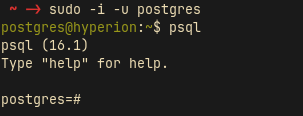
\includegraphics[scale=0.8]{psql.png}
  \caption{\small{Tampilan Terminal PostgreSQL}}
\end{figure}

\subsection{Studi Kasus Perencanaan Basis Data}

\subsubsection{Kasus}

Sebuah universitas ingin mengembangkan sistem basis data akademik untuk menyimpan informasi mahasiswa, mata kuliah, jurusan, serta nilai yang diperoleh mahasiswa. Universitas memiliki aturan sebagai berikut:

\begin{enumerate}
  \item Mahasiswa memiliki ID unik, nama, dan jurusan tempat mereka terdaftar.
  \item Jurusan memiliki ID unik dan nama jurusan.
  \item Mata Kuliah memiliki ID unik, nama mata kuliah, dan jumlah SKS.
  \item Setiap mahasiswa dapat mengambil banyak mata kuliah, dan setiap mata kuliah dapat diambil oleh banyak mahasiswa.
  \item Nilai diberikan kepada mahasiswa berdasarkan mata kuliah yang diambil, dan setiap mahasiswa memiliki satu nilai untuk setiap mata kuliah.
  \item Sistem harus bisa menampilkan laporan mahasiswa beserta jurusan, mata kuliah yang diambil, dan nilai yang diperoleh.
\end{enumerate}

\newpage

\subsubsection{Diagram ERD}

Dari studi kasus, dapat dibentuk ERD atau \emph{Entity Relationship Diagram} sebagai
berikut

\begin{figure}[h]
  \centering
  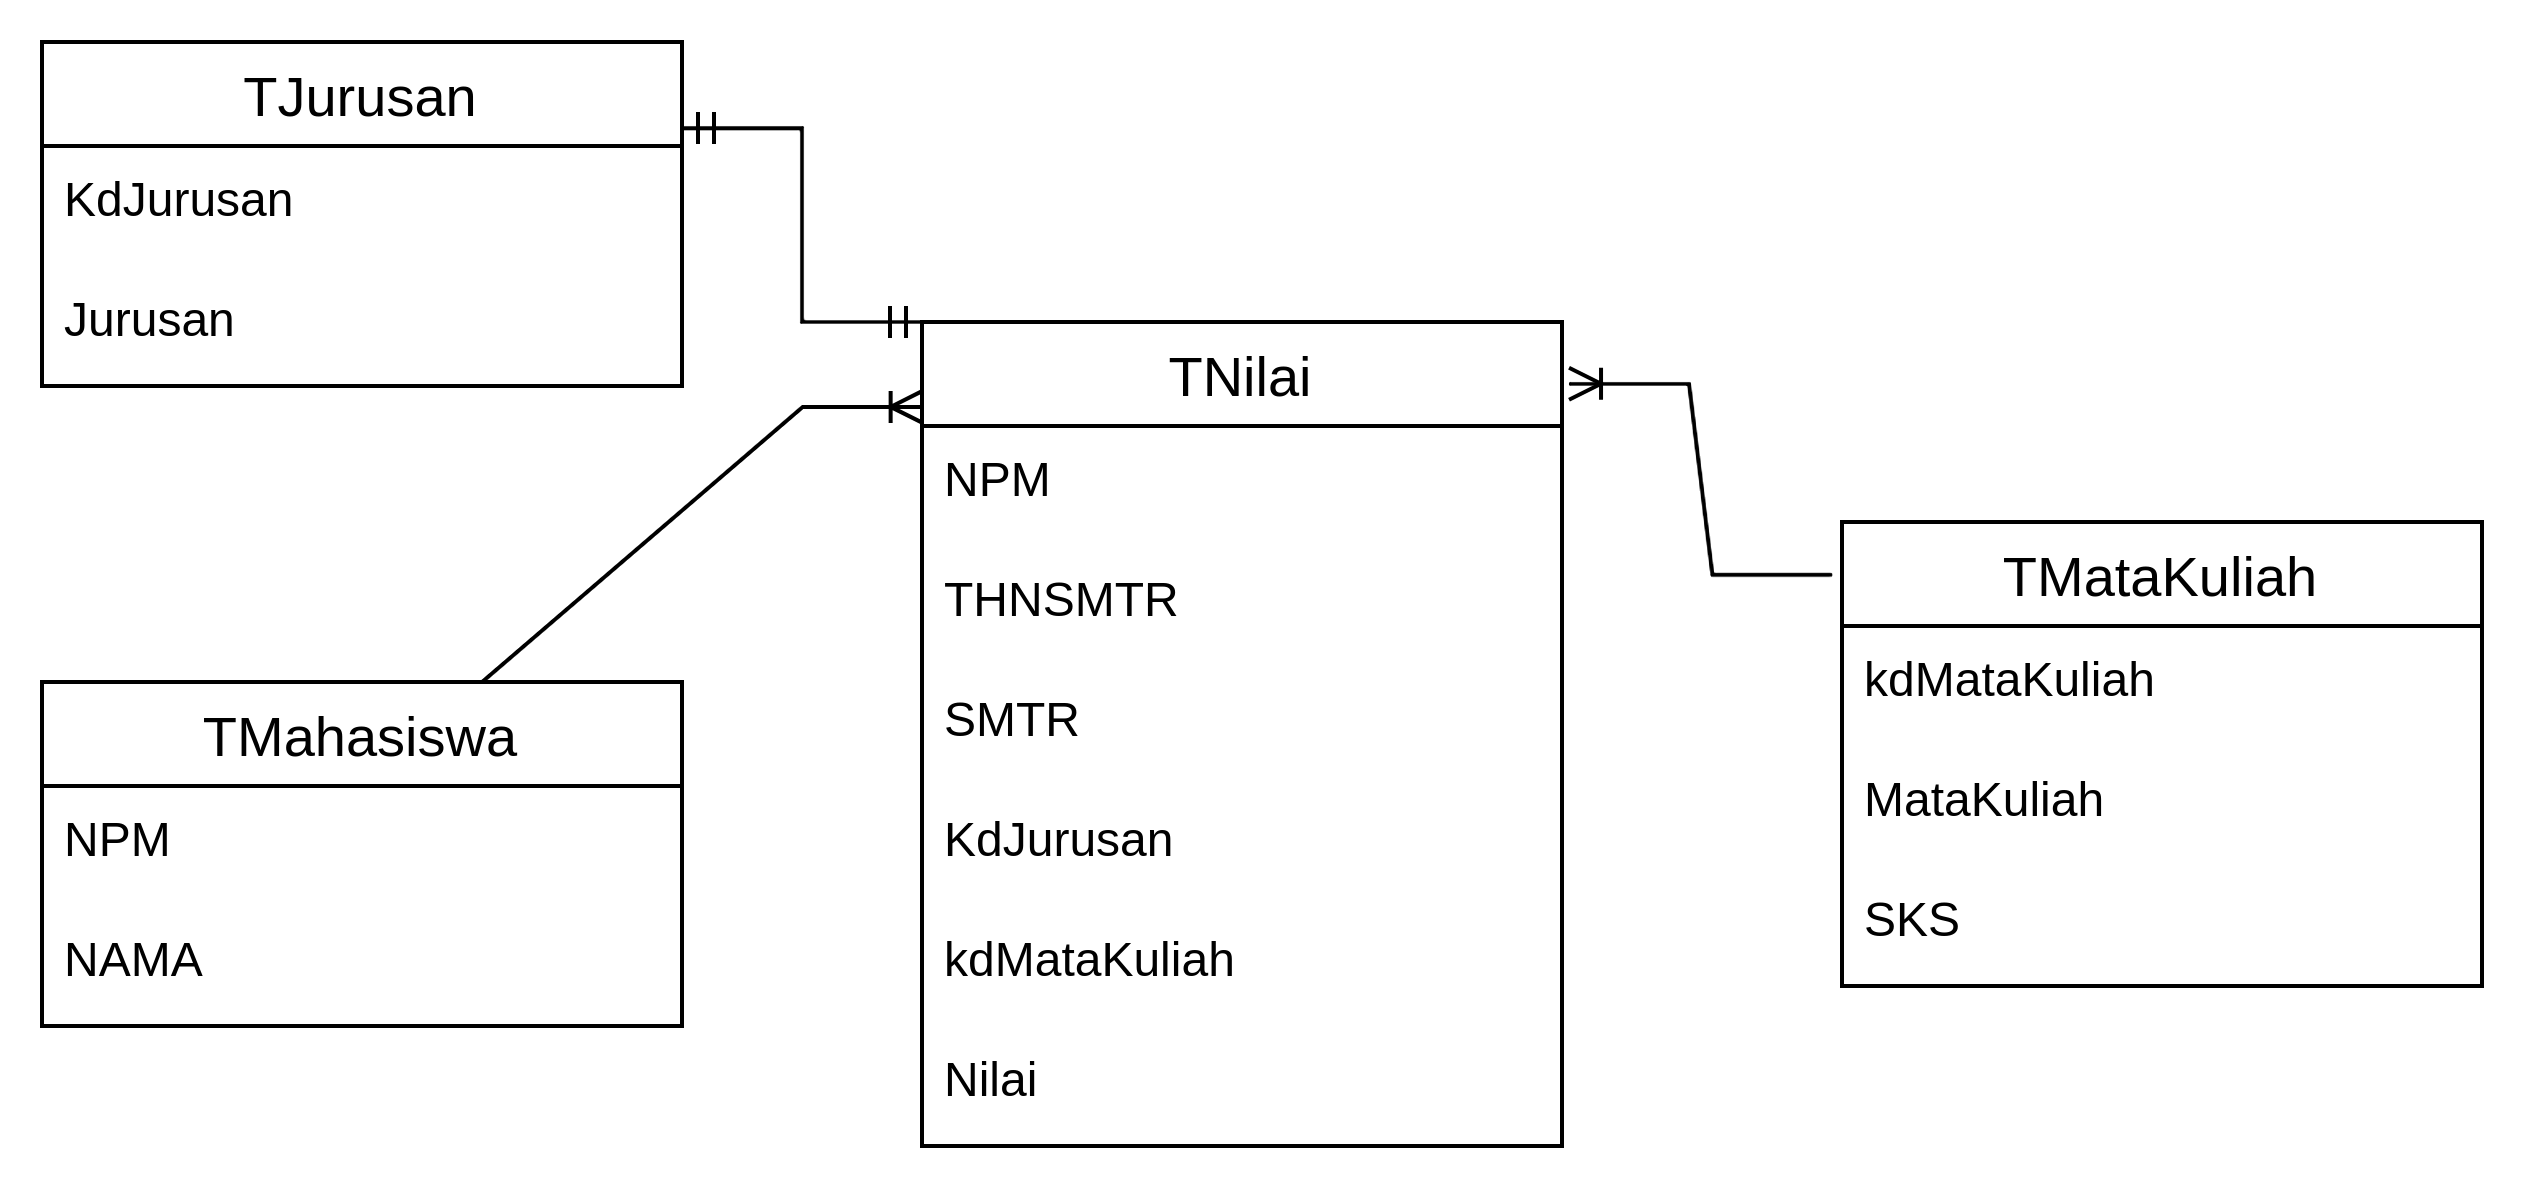
\includegraphics[scale=0.2]{ERD1.png}
  \caption{\small{Diagram ERD dari kasus}}
\end{figure}

\subsubsection{Normalisasi Data}

\cite{normtelkom} ``Normalisasi database adalah proses pengorganisasian data
dalam suatu basis data untuk mengurangi redudansi dan meningkatkan integritas
data.``

Terdapat beberapa tingkatan normalisasi yang dapat dilakukan, masing-masing
memiliki syarat atau kriteria yang harus dipenuhi, antara lain.

\begin{enumerate}
  \item 1NF
    \begin{enumerate}
      \item Tidak memiliki atribut multi-value (tidak ada kelompok-kelompok data yang berulang)
      \item Setiap sel hanya memiliki satu nilai tunggal yang unik
    \end{enumerate}

  \item 2NF
    \begin{enumerate}
      \item Seluruh atribut harus bergantung pada Primary Key
      \item Bila ditemuai adanya ketergantungan parsial, maka atribut tersebut harus di pisah di table lain dan harus dibantu dengan foreign key
    \end{enumerate}

  \item 3NF

    Tidak ada ketergantungan transitif (atribut bukan kunci bergantung pada atribut kunci lainnya)

  \item BCNF (Boyce-Codd Normal Form)

    Bentuk normal Boyce-Codd adalah penyempurnaan dari 3NF di mana tabel harus memenuhi 3NF dan setiap determinan adalah kunci super (superkey).

  \item 4NF

    Tabel berada pada bentuk normal keempat jika sudah memenuhi BCNF dan tidak ada ketergantungan multi-nilai. Pada tingkatan ini, tabel yang memiliki ketergantungan multi-nilai dipecah menjadi tabel-tabel yang lebih kecil untuk menghilangkan anomali.

  \item 5NF

    Bentuk normal kelima berkaitan dengan ketergantungan gabungan. Tabel berada pada bentuk normal kelima jika sudah memenuhi 4NF dan semua ketergantungan gabungan yang ada telah diselesaikan.

\end{enumerate}

Dari ERD studi kasus yang telah dibuat dapat dilihat bahwa data sudah cukup normal, tidak
banyak redudansi yang terjadi. Namun bisa dilakukan setidaknya satu
kali normalisasi. 

Pertama, data yang saat ini dimiliki bisa dinilai adalah bentuk normal 2, karena
sudah terdapat primary key yang membentuk relasi. Data tabel bisa divisualisasi
sebagai berikut.

\vspace{1cm}

\begin{adjustbox}{scale=0.5,center}
  \begin{tabular}{ |c|c|c|c|c|c| } 
    \hline
    \multicolumn{6}{|c|}{Tabel Nilai} \\ \hline
    NPM        & THNSMTR   & SMTR    & kode jurusan & KodeMkl & Nilai \\ \hline \hline
    6020218001 & 2019/2020 & Genap   & 60202        & MKDU-15 & A     \\ \hline
    6020218001 & 2018/2020 & Ganjl   & 60202        & MKDU-13 & A     \\ \hline
    6020218001 & 2020/2020 & Ganjil  & 60203        & MKDU-15 & A     \\ \hline
    6020218002 & 2019/2020 & Ganjil  & 60203        & MKDU-16 & A     \\ \hline
    6020218002 & 2018/2020 & Genap   & 60203        & MKDU-39 & A     \\ \hline
    6020218002 & 2019/2020 & Genap   & 60203        & MKDU-21 & A     \\ \hline
    6020218002 & 2018/2019 & Genap   & 60202        & MKDU-12 & A     \\ \hline
    6020218003 & 2020/2021 & Ganjil  & 60202        & MKDU-23 & A     \\ \hline
    6020218003 & 2019/2020 & Genap   & 60202        & MKDU-14 & A     \\ \hline
    6020218003 & 2019/2020 & Ganjil  & 60202        & MKDU-11 & A     \\ 
    \hline
  \end{tabular}
\end{adjustbox}

\begin{multicols}{3}
  \begin{adjustbox}{scale=0.5,center}
    \begin{tabular}{ |c|c|c| } 
      \hline
      \multicolumn{3}{|c|}{Tabel Matakuliah}  \\ \hline
      KodeMkl & Matakuliah                    & SKS \\ \hline \hline
      MKDU-11 & Ishul Fiqh                    & 2  \\ \hline                                    
      MKDU-12 & Fiqh Muamalah I               & 2  \\ \hline                                    
      MKDU-13 & Filsafat Ilmu           	    & 2  \\ \hline                                    
      MKDU-14 & Fiqh Muamalah III             & 2  \\ \hline                                    
      MKKU-15 & Kaidah Fiqh Muamalah          & 3  \\ \hline                                    
      MKDU-15 & Pendidikan Anti Korupsi       & 2  \\ \hline                                    
      MKDU-16 & Ekonomi Mikro Islam I         & 2  \\ \hline                                    
      MKDU-21 & Fiqh Lembaga Keuangan Syariah & 3  \\ \hline                                    
      MKDU-23 & Filsafat Ekonomi Islam        & 2  \\ \hline                                    
      MKDU-39 & Teknik Penulisan Karya Ilmiah & 2  \\ \hline
    \end{tabular}
  \end{adjustbox}

  \begin{adjustbox}{scale=0.6,center}
    \begin{tabular}{ |c|c| } 
      \hline
      \multicolumn{2}{|c|}{Tabel Jurusan} \\ \hline
      kode Jurusan  & Jurusan           \\ \hline \hline
      60202         & Ekonomi Syariah   \\ \hline
      60203         & Akutansi Syariah  \\ \hline
    \end{tabular}
  \end{adjustbox}

  \columnbreak

  \begin{adjustbox}{scale=0.6,center}
    \begin{tabular}{ |c|c| } 
      \hline \multicolumn{2}{|c|}{Tabel Mahasiswa} \\ \hline
      NPM        & NAMAMHS   \\ \hline \hline
      6020218001 & Ai Supita \\ \hline
      6020218002 & Rendi     \\ \hline
      6020218003 & Hanifa    \\ \hline
    \end{tabular}
  \end{adjustbox}

\end{multicols}

\begin{figure}[h]
  \centering
  \caption{\small{Normal 2}}
\end{figure}

Di visualisasi data diatas, dapat diamati bahwa tabel nilai memiliki data
berulang yaitu data mengenai jurusan dan mata kuliah. Informasi tersebut
dapat dipisah lagi kedalam tabel tambahan agar mengurangi redudansi dan
menghilangkan ketergantungan non kunci atau transitif, hingga didapatkan
bentuk yang memenuhi kriteria normal 3.

\vspace{1cm}

\begin{adjustbox}{scale=0.5,center}
  \begin{tabular}{ |c|c|c|c|c| } 
    \hline
    \multicolumn{5}{|c|}{Tabel Nilai} \\ \hline
    NPM        & THNSMTR   & SMTR    &  KodeMkl & Nilai \\ \hline \hline
    6020218001 & 2019/2020 & Genap   &  MKDU-15 & A     \\ \hline
    6020218001 & 2018/2020 & Ganjl   &  MKDU-13 & A     \\ \hline
    6020218001 & 2020/2020 & Ganjil  &  MKDU-15 & A     \\ \hline
    6020218002 & 2019/2020 & Ganjil  &  MKDU-16 & A     \\ \hline
    6020218002 & 2018/2020 & Genap   &  MKDU-39 & A     \\ \hline
    6020218002 & 2019/2020 & Genap   &  MKDU-21 & A     \\ \hline
    6020218002 & 2018/2019 & Genap   &  MKDU-12 & A     \\ \hline
    6020218003 & 2020/2021 & Ganjil  &  MKDU-23 & A     \\ \hline
    6020218003 & 2019/2020 & Genap   &  MKDU-14 & A     \\ \hline
    6020218003 & 2019/2020 & Ganjil  &  MKDU-11 & A     \\ 
    \hline
  \end{tabular}
\end{adjustbox}

\begin{multicols}{3}
  \begin{adjustbox}{scale=0.5,center}
    \begin{tabular}{ |c|c| } 
      \hline
      \multicolumn{2}{|c|}{Tabel JurusanMatakuliah}  \\ \hline
      KodeMkl & kode jurusan \\ \hline \hline
      MKDU-11 & 60202        \\ \hline                                    
      MKDU-12 & 60202        \\ \hline                                    
      MKDU-13 & 60203        \\ \hline                                    
      MKDU-14 & 60203        \\ \hline                                    
      MKKU-15 & 60203        \\ \hline                                    
      MKDU-15 & 60203        \\ \hline                                    
      MKDU-16 & 60202        \\ \hline                                    
      MKDU-21 & 60202        \\ \hline                                    
      MKDU-23 & 60202        \\ \hline                                    
      MKDU-39 & 60202        \\ \hline
    \end{tabular}
  \end{adjustbox}

  \begin{adjustbox}{scale=0.5,center}
    \begin{tabular}{ |c|c|c| } 
      \hline
      \multicolumn{3}{|c|}{Tabel Matakuliah}  \\ \hline
      KodeMkl & Matakuliah                    & SKS \\ \hline \hline
      MKDU-11 & Ishul Fiqh                    & 2  \\ \hline                                    
      MKDU-12 & Fiqh Muamalah I               & 2  \\ \hline                                    
      MKDU-13 & Filsafat Ilmu           	    & 2  \\ \hline                                    
      MKDU-14 & Fiqh Muamalah III             & 2  \\ \hline                                    
      MKKU-15 & Kaidah Fiqh Muamalah          & 3  \\ \hline                                    
      MKDU-15 & Pendidikan Anti Korupsi       & 2  \\ \hline                                    
      MKDU-16 & Ekonomi Mikro Islam I         & 2  \\ \hline                                    
      MKDU-21 & Fiqh Lembaga Keuangan Syariah & 3  \\ \hline                                    
      MKDU-23 & Filsafat Ekonomi Islam        & 2  \\ \hline                                    
      MKDU-39 & Teknik Penulisan Karya Ilmiah & 2  \\ \hline
    \end{tabular}
  \end{adjustbox}

  \begin{adjustbox}{scale=0.6,center}
    \begin{tabular}{ |c|c| } 
      \hline
      \multicolumn{2}{|c|}{Tabel Jurusan} \\ \hline
      kode Jurusan  & Jurusan           \\ \hline \hline
      60202         & Ekonomi Syariah   \\ \hline
      60203         & Akutansi Syariah  \\ \hline
    \end{tabular}
  \end{adjustbox}

  \columnbreak

  \begin{adjustbox}{scale=0.6,center}
    \begin{tabular}{ |c|c| } 
      \hline \multicolumn{2}{|c|}{Tabel Mahasiswa} \\ \hline
      NPM        & NAMAMHS   \\ \hline \hline
      6020218001 & Ai Supita \\ \hline
      6020218002 & Rendi     \\ \hline
      6020218003 & Hanifa    \\ \hline
    \end{tabular}
  \end{adjustbox}


\end{multicols}

\begin{figure}[h]
  \centering
  \caption{\small{Normal 3}}
\end{figure}

Dibentuk normal 3 ini, sudah cukup terminimalisir pengulangan data atau
redudansi, hingga sudah tidak perlu dilakukan normalisasi lebih lanjut.

\begin{figure}[h]
  \centering
  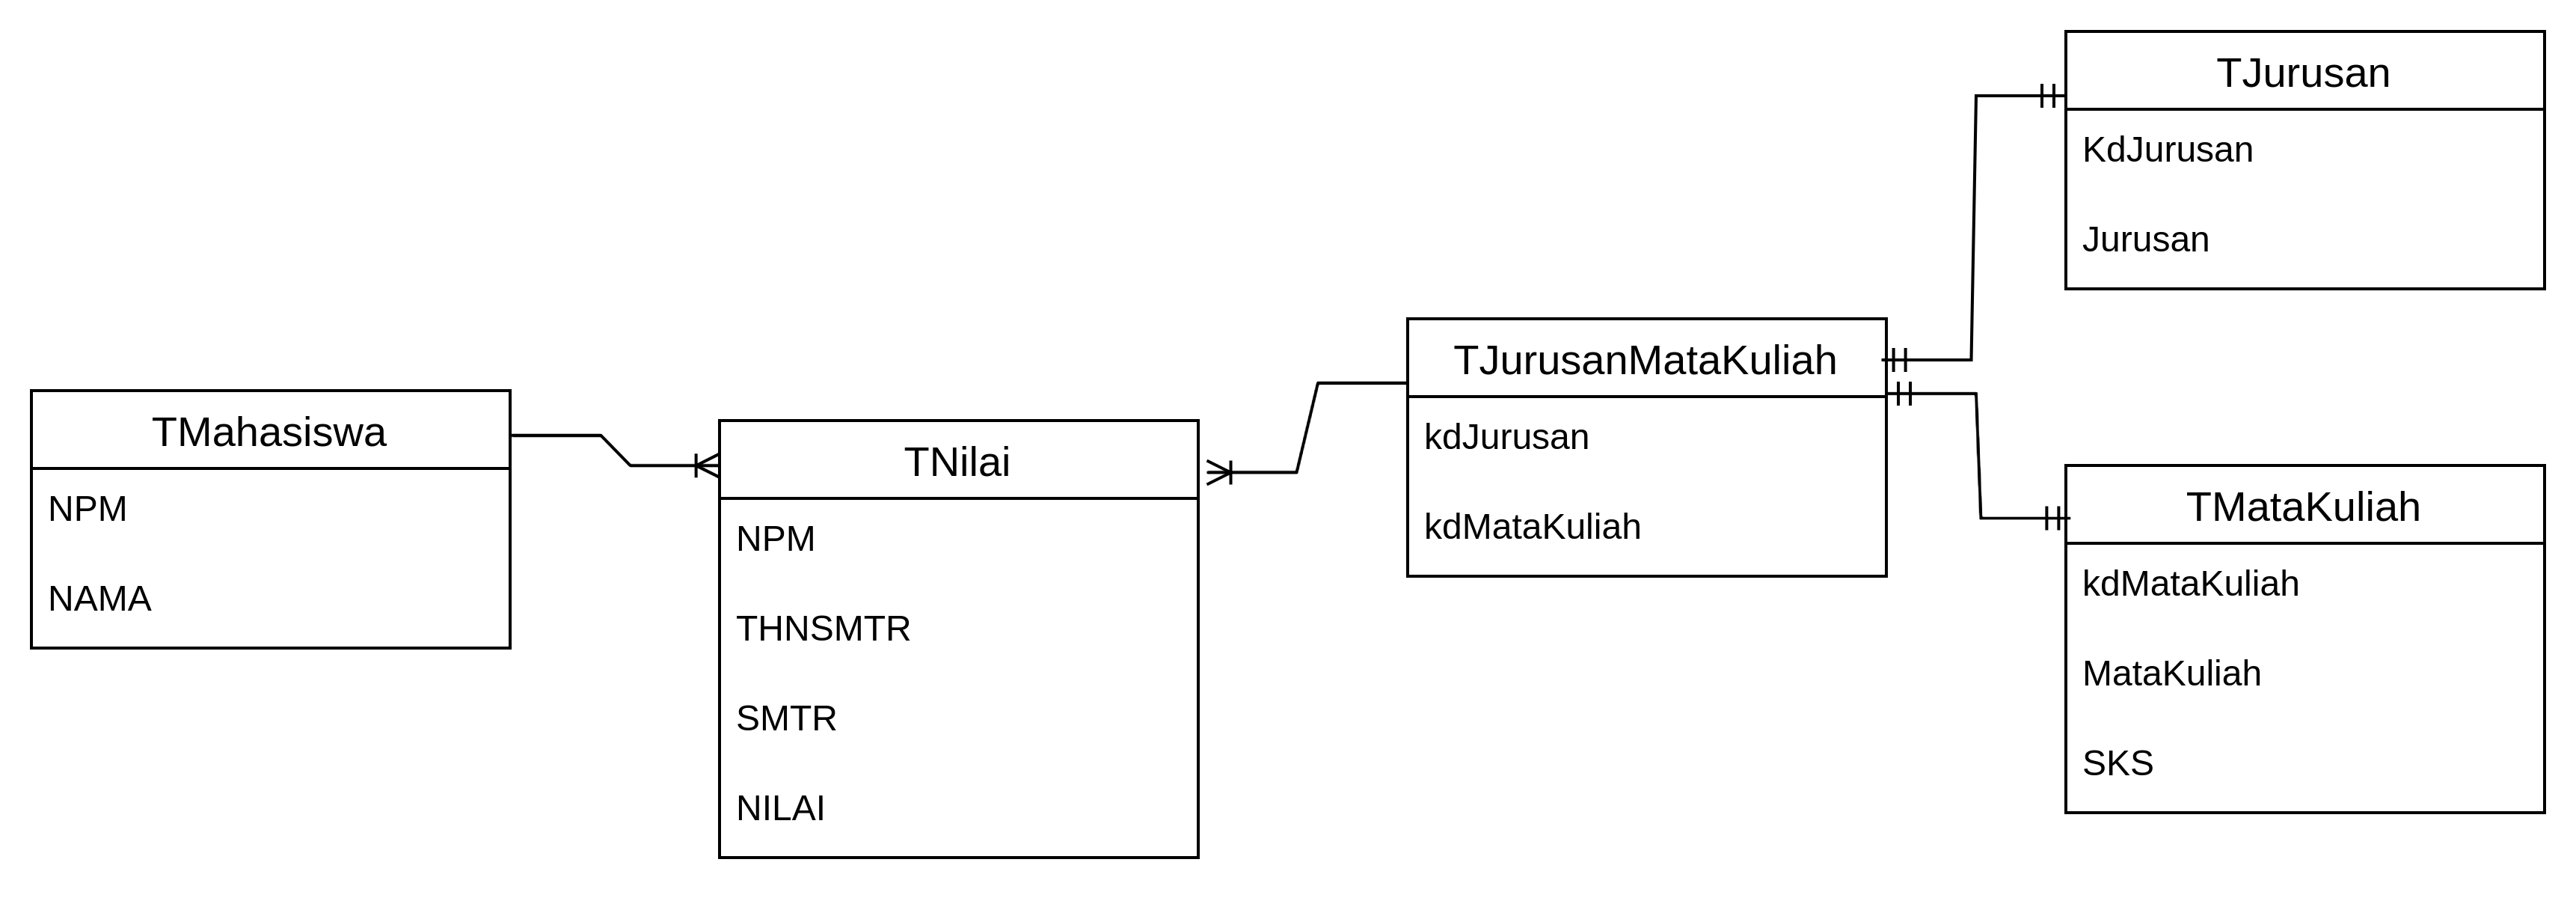
\includegraphics[scale=0.19]{ERD2.png}
  \caption{\small{Diagram ERD Setelah Normalisasi}}
\end{figure}

\newpage 

\begin{center}

  \large{\textbf{BAB III}}

  \section*{KESIMPULAN}

\end{center}

\addcontentsline{toc}{section}{BAB III KESIMPULAN}{}

Berdasarkan hasil eksplorasi dan implementasi yang telah dilakukan, dapat
disimpulkan bahwa PostgreSQL merupakan sistem manajemen basis data yang
handal, fleksibel, dan sesuai untuk berbagai kebutuhan pengolahan data.
PostgreSQL menawarkan fitur-fitur unggulan seperti dukungan terhadap ACID
(Atomicity, Consistency, Isolation, Durability), sistem Object-Relational 
Database, serta kemampuan ekstensibilitas yang tinggi melalui fungsi-fungsi
kustom dan dukungan berbagai bahasa pemrograman.

Dalam studi kasus yang telah dibahas, perancangan basis data dilakukan
dengan menerapkan prinsip normalisasi untuk memastikan efisiensi
penyimpanan dan integritas data.

Dengan demikian, PostgreSQL dapat menjadi solusi yang efektif dalam 
pengelolaan basis data yang kompleks. Penggunaan dan optimasi lebih
lanjut dapat terus dikembangkan sesuai dengan kebutuhan sistem dan
organisasi yang menggunakannya.

\newpage 

\begin{center}
  \section*{DAFTAR PUSTAKA}
\end{center}

\setcounter{section}{1}

\setcounter{subsection}{0}

\addcontentsline{toc}{section}{DAFTAR PUSTAKA}{}

\pagenumbering{gobble}


\bibliographystyle{plain}
\bibliography{./src/TugasLaporanPostgreql} 

  \end{document}
